%%
%% Author: dariochinelli
%% 2019-12-04
%%

% Preamble
\documentclass[class=article, crop=false]{standalone}

% Packages
\usepackage{tikz}
\usetikzlibrary{positioning}

% Document
\begin{document}


\begin{figure}[h!]
\centering
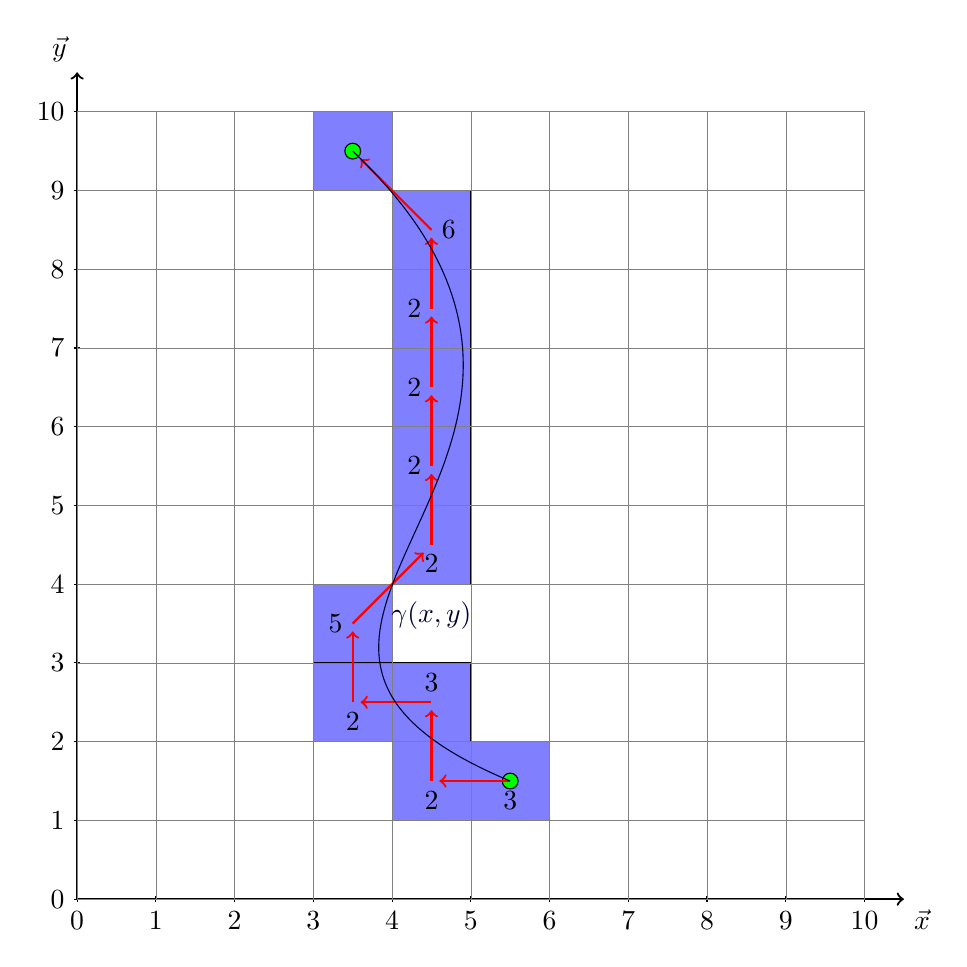
\begin{tikzpicture}

% Title
%% \draw (0,-0.6) -- (10,-0.6) node[midway,below] {eg of a trajectory and K for each positions};
%% \draw (0,-1.1) -- (10,-1.1);

% Axis lines
\draw[thick,->] (0,0) -- (10.5,0) node[anchor=north west] {$\vec x$};
\draw[thick,->] (0,0) -- (0,10.5) node[anchor=south east] {$\vec y$};

% Nodes
\foreach \x in {0,1,2,3,4,5,6,7,8,9,10}
   \draw (\x cm,1pt) -- (\x cm,-1pt) node[anchor=north] {$\x$};
\foreach \y in {0,1,2,3,4,5,6,7,8,9,10}
\draw (1pt,\y cm) -- (-1pt,\y cm) node[anchor=east] {$\y$};

% Color
\filldraw[fill=blue!50!white] (4,1) rectangle (6,2);
\filldraw[fill=blue!50!white] (3,2) rectangle (5,3);
\filldraw[fill=blue!50!white] (3,3) rectangle (4,4);
\filldraw[fill=blue!50!white] (4,4) rectangle (5,9);
\filldraw[fill=blue!50!white] (3,9) rectangle (4,10);

% Grid
\draw[step=1cm,gray,very thin] (0,0) grid (10,10);
\draw[fill=green] (5.5,1.5) circle (0.1cm);
\draw[fill=green] (3.5,9.5) circle (0.1cm);

% Lines
\draw[thick,->,red] (5.5,1.5) node[black,below] {3} -- (4.6,1.5);
\draw[thick,->,red] (4.5,1.5) node[black,below] {2} -- (4.5,2.4);
\draw[thick,->,red] (4.5,2.5) node[black,above] {3} -- (3.6,2.5);
\draw[thick,->,red] (3.5,2.5) node[black,below] {2} -- (3.5,3.4);
\draw[thick,->,red] (3.5,3.5) node[black,left] {5} -- (4.4,4.4);
\draw[thick,->,red] (4.5,4.5) node[black,below] {2} -- (4.5,5.4);
\draw[thick,->,red] (4.5,5.5) node[black,left] {2} -- (4.5,6.4);
\draw[thick,->,red] (4.5,6.5) node[black,left] {2} -- (4.5,7.4);
\draw[thick,->,red] (4.5,7.5) node[black,left] {2} -- (4.5,8.4);
\draw[thick,->,red] (4.5,8.5) node[black,right] {6} -- (3.6,9.4);

\draw[blue!20!black] (5.5,1.5) .. controls (0.95,3.4) and (7.6,5.6) .. (3.5,9.5);
\node[blue!20!black] at (4.5,3.6) {$\gamma(x, y)$};

\end{tikzpicture}
\captionsetup{width=.8\linewidth}
\caption{This illustration represents a trajectory in the \emph{continuous space} as the blue line $\gamma$.
That path $\gamma$ is discretized in the \emph{grid space}, represented by the blue cells.
The red arrows represents the change from a cell to the next.
The numbers are the associated to the D2Q9 indexes to those moves, also called \emph{k-directions}}

\label{illustrate_eg_path}
\end{figure}


\end{document}
